
\documentclass[titlepage]{article}
 \usepackage[utf8]{inputenc}
\usepackage{listings}
\usepackage{hyperref}
\usepackage{float}
\usepackage{graphicx}
\usepackage{subfig}
\graphicspath{ {imagenes/} }
 \usepackage{xcolor}
 \definecolor{RoyalBlue}{cmyk}{1, 0.50, 0, 0}

\lstset{language=Java,
	keywordstyle=\color{RoyalBlue},
	basicstyle=\scriptsize\ttfamily,
	commentstyle=\ttfamily\itshape\color{gray},
	stringstyle=\ttfamily,
	showstringspaces=false,
	breaklines=true,
	frameround=ffff,
	frame=single,
	rulecolor=\color{black}}


 

% Datos de la portada
\begin{document}
	

	\section{Regresión logística(RL)}	
	En este caso nos hemos decantado por RL porque fue el modelo que mejor resultados nos dio en la practica pasada, y al ser un dataset de datos que trata un modelo parecido podremos utilizar los conocimientos previos para mejorarlo. En este caso como el problema es multiclase se ha utilizado one vs rest para clasificar. Vamos a realizar una pequeña explicación de como funciona.
	
	Vamos a poner un pequeño ejemplo con tres clases para ver como funcionaria. Como se ve en la siguiente imagen es imposible dividir las clases con una única linea. 
	\begin{figure}[H]
		\centering
		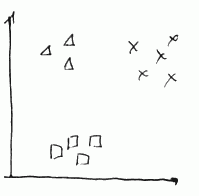
\includegraphics[width=0.7\linewidth]{../imagenesRL/screenshot002}
		\caption{Conjunto de clases}
		\label{fig:screenshot002}
	\end{figure}
	
	En las siguientes imágenes se ve como enfrentamos una clase a las otras dos de forma que si se puede conseguir una separación mediante una función lineal.
	
	
	
	\begin{figure}[H]
		\centering
		\subfloat[Triangulos]{
			\label{f:gato}
			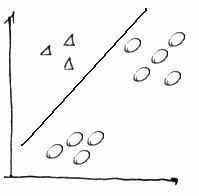
\includegraphics[width=0.3\textwidth]{../imagenesRL/screenshot001}}
		\subfloat[Cuadrados]{
			\label{f:tigre}
			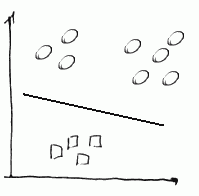
\includegraphics[width=0.3\textwidth]{../imagenesRL/screenshot004}}
		\subfloat[Cruces]{
			\label{f:conejo}
			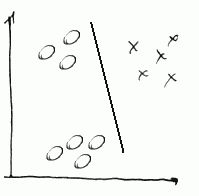
\includegraphics[width=0.3\textwidth]{../imagenesRL/screenshot005}}
		\caption{División mediante one vs rest}
	\end{figure}
	
	\subsection{Especificación de parámetros RL}
	Los parametros a tener en cuenta son:
	\begin{enumerate}		
		\item{Umbral de parada:} Indicara cuando tengamos un error menor al indicado pararemos.
		\item{Numero de iteraciones máxima:} En este caso sera en numero máximo de iteraciones podrá realizar si no decide parar antes por el umbral de parada.
	\end{enumerate}
	Para estos parámetros hemos utilizados los valores por defecto dados por la librería sklean con la que se ha realizado la practica. En este caso el numero de iteraciones esta fijado a 100, aunque suele parar antes sobre unas 30 o 40 iteraciones y el umbral de parada esta inicializado a $10^{-4}$.
	
	En este caso se han realizado pruebas para obtener el mejor parámetro(C) para la regularización. Este parámetro a medida que aumenta realiza una regularización mas suave. También se han realizado pruebas con dos tipos de regularización, que son la L1 y L2. 
	
	\begin{figure}[H]
		\centering
		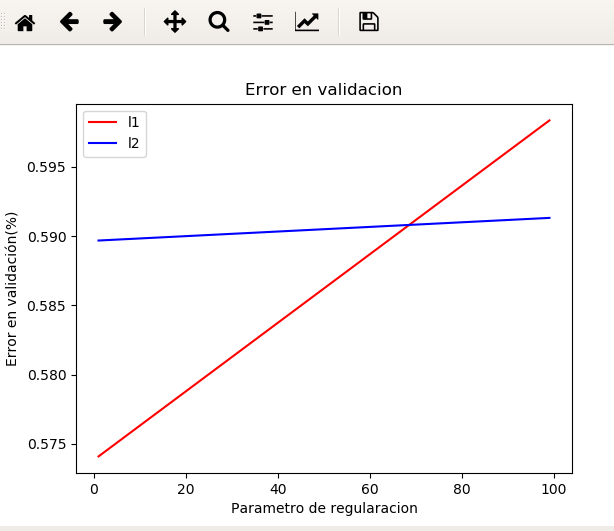
\includegraphics[width=0.7\linewidth]{../imagenesRL/graficaRegularizacion}
		\caption{}
		\label{fig:Grafica de regularizacion}
	\end{figure}

	En este caso se ve como l1 consigue superar a l2 a la hora de ajustar el error en la partición de validación aunque la mejora solo son en torno a un 0.03\%. En este caso no es muy notorio. El problema viene dado a la hora de tener en cuenta el tiempo de ejecución entre una y otra. 
	\begin{figure}[H]
		\centering
		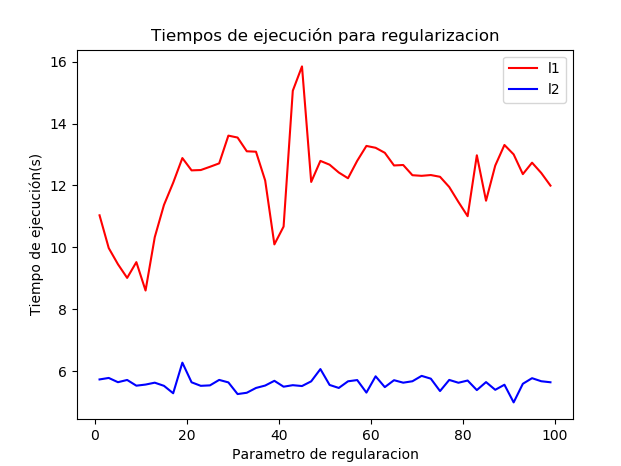
\includegraphics[width=0.7\linewidth]{../imagenesRL/tiemposEjecucion}
		\caption{}
		\label{fig:tiemposejecucion}
	\end{figure}
En este caso l2 es bastante superior a l1. Por estos motivos he decido un parámetro C de 100 y utilizar la regularización de L2.
	
	\subsection{Valoración de resultados}
	En este caso para le medición del error se ha utilizado es el mean accuracy.
	Se consigue en la partición de test un Eout del 2.3727\% en un tiempo de 4.9801 segundos. Vamos a revisar la matriz de confusión para ver mas información.
	
	\begin{figure}[H]
		\centering
		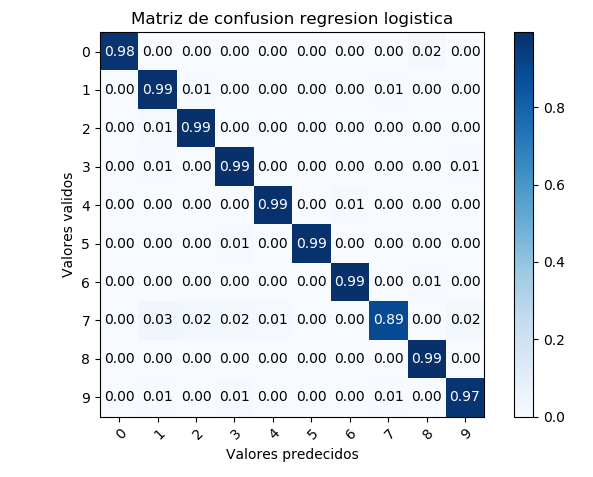
\includegraphics[width=0.7\linewidth]{../imagenesRL/matrizconfusion}
		\caption{}
		\label{fig:Matriz confusion RL}
	\end{figure}

	En este caso se tiene un 10\% errores al adivinar el numero 7, confundiendo este con 1, 2 y 3 . Esto haría que aunque el modelo en geneal tenga un buen acierto se tenga problemas al equivocarnos a menudo en el numero 7.
	
	
	





\end{document}

